% arara: xelatex
% arara: biber
% arara: xelatex
% arara: xelatex

\documentclass[twoside,12pt,openany]{book}

%%%%%%%%%%%%%%%%%%%%%%%%%%%%%%%%%%%%%%%%%%%%%%%%%%%%%%%%%%
% define author's name and document title
\def\theauthor{Nithiya Mangala Streethran}
\def\thetitle{%
  Specification of \texorpdfstring{`}{'}normal' wind turbine operating
  behaviour for rapid anomaly detection:\texorpdfstring{\\}{}
  through the use of machine learning algorithms%
}

% PDF metadata - optional subject and comma-separated keywords
% leave the braces blank if not applicable
\def\subject{Renewable Energy Engineering}
\def\keywords{%
  wind turbine, classification algorithm, SCADA, fault detection,
  condition monitoring%
}

% choose internal and external link colours
% (named colours via svgnames are available)
% see xcolor's documentation for a full list of svgnames colours:
% http://mirrors.ctan.org/macros/latex/contrib/xcolor/xcolor.pdf
\def\externallink{SeaGreen}
\def\internallink{DarkOrchid}

\usepackage{docstyle}
\addbibresource{references.bib}

\begin{document}
%%%%%%%%%%%%%%%%%%%%%%%%%%%%%%%%%%%%%%%%%%%%%%%%%%%%%%%%%%

\frontmatter

% use \maketitle, or define a custom titlepage
\begin{titlepage}
  \hspace{0pt}\vfill % vertical centering
  \centering % horizontal centering
  \Large\thetitle
  \\[4cm]
  \large\theauthor
  \vfill
  25th August 2017
  \\[.5cm]
  Last updated: \today
  \vfill\hspace{0pt} % vertical centering
\end{titlepage}

% copyright info
\hspace{0pt}\vfill
\noindent\textcopyright~2017-\the\year{}~\theauthor \\[.5cm]
\noindent Email: nmstreethran@gmail.com \\[.5cm]
\noindent The contents of this document are licensed under a
\href{https://creativecommons.org/licenses/by/4.0/}%
{Creative Commons Attribution 4.0 International (CC-BY-4.0) License}.
\vfill\hspace{0pt}

\onehalfspacing

%%%%%%%%%%%%%%%%%%%%%%%%%%%%%%%%%%%%%%%%%%%%%%%%%%%%%%%%%%
\chapter*{Abstract}

Maximising the economic effectiveness of a wind farm is essential in making
wind a more economic source of energy. This effectiveness can be increased
through the reduction of operation and maintenance costs, which can be
achieved through continuously monitoring the condition of wind turbines. An
alternative to expensive condition monitoring systems, which can be
uneconomical especially for older wind turbines, is to implement
classification algorithms on supervisory control and data acquisition (SCADA)
signals, which are collected in most wind turbines. Several publications were
reviewed, which were all found to use separate algorithms to predict specific
faults in advance. In reality, wind turbines tend to have multiple faults
which may happen simultaneously and have correlations with one another. This
project focusses on developing a methodology to predict multiple wind turbine
faults in advance simultaneously by implementing classification algorithms on
SCADA signals for a wind farm with 25 turbines rated at 2,500 kW, spanning a
period of 30 months. The data, which included measurements of wind speed,
active power and pitch angle, was labelled using corresponding downtime data
to detect normal behaviour, faults and varying timescales before a fault
occurs. Three different classification algorithms, namely decision trees,
random forests and k nearest neighbours were tested using imbalanced and
balanced training data, initially to optimise a number of hyperparameters. The
random forest classifier produced the best results. Upon conducting a more
detailed analysis on the performance of specific faults, it was found that the
classifier was unable to detect the varying timescales before a fault with
accuracy comparable to that of normal or faulty behaviour. This could have
been due to the SCADA data, which are used as features, being unsuitable for
detecting the faults, and there is potential to improve this by balancing only
these classes.

\noindent\textbf{\textit{Keywords:}} \keywords

\contentlists

\themainmatter

\chapter{Introduction}\label{c1}

\section{Background}

There is a need to increase the economic effectiveness of wind turbines, which
refers to the cost to run them relative to the electricity generation, or
revenue \cite{Kim12,Leahy16}. Increasing this effectiveness lowers the payback
period of new wind turbines or farms, thus making wind a more economic clean
energy source, attracting governments and private organisations to make more
investments in wind projects \cite{Kim12}. It can, however, be decreased due
to major component failure, frequent downtime, turbine degradation and age,
which in turn increase the operation and maintenance cost and decrease the
energy generation efficiency of wind turbines \cite{Kim12,Diens16}. There are
difficulties and high costs involved in carrying out maintenance on wind
turbines, especially for ones that operate in extreme and remote conditions,
such as offshore wind farms, where the turbines tend to also exist in larger
numbers \cite{Diens16,Tautz17}.

Condition-based monitoring systems that continuously monitor wind turbine
states increase this effectiveness by significantly reducing the maintenance
costs, reportedly by 20\,\% to 25\.\%, as it prevents unscheduled maintenance
\cite{Leahy16}. According to the Electric Power Research Institute, reactive
maintenance, which refers to running the turbine until it reaches failure, has
the highest cost, followed by preventive or scheduled maintenance, which is
reported to cost 24\,\% less \cite{Wind15}. Meanwhile, condition-based or
predictive maintenance, which prevents catastrophic failure, \cite{Kim12} is
reported to save 47\,\% of the cost of reactive maintenance, \cite{Wind15}
which makes it the most cost-effective and preferred approach. Condition-based
monitoring technologies include sensor-based oil and vibration analysis, which
are useful for checking the oil for properties such as temperature, and
rotating equipment, respectively \cite{Garci12}. These technologies, however,
tend to put emphasis on the more expensive parts of a wind turbine such as the
gearbox \cite{Godwi13} due to the high costs involved in the installation of
these sensors \cite{Leahy16,Garci12}. These systems, which can be purchased
from the turbine manufacturer, are usually pre-installed in offshore wind
turbines due to the harsh environments in which they operate. However, they
can be expensive \cite{Tautz17} and uneconomical, especially for older wind
turbines in onshore wind farms, whose outputs are often less than that of an
offshore wind farm.

An alternative would be to use SCADA-based analysis, where the only cost
involved would be computational and expensive sensors are not required
\cite{Leahy16,Tautz17}. A SCADA system, which stands for supervisory control
and data acquisition, found pre-installed in most utility-scale wind turbines,
collects data using numerous sensors at the controllers with usually 10-minute
resolution \cite{Tautz17,Yang14}, of various parameters of the wind turbine,
such as wind speed, active power, bearing temperature and voltage
\cite{Leahy16}. Power curve analysis can be done using this data, but this
analysis only detects wind turbine underperformance \cite{Gill12}. Meanwhile,
implementing machine learning algorithms on SCADA signals to classify them as
having either normal or anomalous behaviour, has the ability to predict faults
in advance. This has been demonstrated in a number of publications.

Kusiak and Li \cite{Kusia11} investigated predicting a specific fault, which
is diverter malfunction. 3 months' worth of SCADA data of four wind turbines
were used and the corresponding status and fault codes were integrated into
this data to be labelled to differentiate between normal and fault points. To
prevent bias in prediction in machine learning, the labelled data is sampled
at random, ensuring the number of samples with a fault code is comparable to
the number of normal samples. Four classification algorithms, namely neural
networks, boosting tree, support vector machines, and classification and
regression trees were trained using two-thirds of this data which was randomly
selected. The boosting tree, which was found to have the highest accuracy of
70\,\% for predicting specific faults, was investigated further. The accuracy
of predicting a specific fault at the time of fault was 70\,\%, which
decreased to 49\,\% for predicting it 1 hour in advance. Only one specific
fault was the focus of this methodology and in reality, wind turbines could
have many faults in different components and structures, which may all have
some form of correlation between one other.

Godwin and Matthews \cite{Godwi13} focussed on wind turbine pitch control
faults using a classifier called the RIPPER algorithm. They used 28 months'
worth of SCADA data containing wind speeds, pitch motor torques and pitch
angles, of eight wind turbines known to have had pitch problems in the past.
The classes used were normal, potential fault and recognised fault. Using
maintenance logs, data up to 48 hours in advance was classed as recognised
fault, data in advance of this with corresponding SCADA alarm logs indicating
pitch problems was classed as potential fault, and the remaining unclassed
data was classed as normal. Random sampling was performed here as well to
balance the classes and prevent bias. The data of four turbines were used to
train the RIPPER algorithm, and the remaining four used for testing. The
analysis was done using the entire 28 months of data as well as 24, 20, 16,
12, 8 and 4 months of data to find out how the amount of data affects the
accuracy of classification. Using the entire 28 months of data was found to
produce the most accurate classifier, with a mean accuracy of 85\,\%. Looking
at the results in more depth, it was found that the classifier had F1 scores,
which is an accuracy measure that accounts for true and false positives and
negatives, of 79\,\%, 100\,\% and 78\,\% in classifying normal, potential
fault and recognised fault data, respectively. Although the results are an
improvement to Kusiak and Li \cite{Kusia11}, this methodology similarly
focussed on only one fault.

Leahy \textit{et al.} \cite{Leahy16} used a specific fault prediction approach,
implementing a support vector machine classifier from scikit-learn's LibSVM.
They used SCADA data from a single 3 MW wind turbine spanning 11 months with
status and warning codes. The labelling was done such that data with codes
corresponding to the turbine in operation, low and storm wind speeds represent
normal conditions and codes corresponding to each specific fault to represent
faulty conditions. Data preceding these fault points by 10 minutes and 60
minutes were also labelled as faults in separate sets and the effects of using
these different time scales to predict faults were investigated. For data
identified as normal, filters were applied to remove curtailment and anomalous
points. The classifier's hyperparameters were optimised using randomised grid
search and validated using ten-fold cross-validation, and the classes were
balanced using class weights. Separate binary classifiers were trained to
detect each specific type of fault, which were faults in air cooling,
excitation, generator heating, feeding and mains failure. The prediction of
generator heating faults 10 minutes in advance had the best results, with F1
scores of 71\,\% and 100\,\% using balanced and imbalanced training data,
respectively. This increase in score using imbalanced data was attributed to
the test set having very few instances with the fault class relative to normal
data. The same fault, when predicted 60 minutes in advance, had F1 scores of
17\,\% and 100\,\% using imbalanced and balanced training data, respectively.
Although the score is perfect and it demonstrates the effects of using
balanced datasets, the classification again is done separately for each
specific fault and it performed poorly on other faults. For instance,
detecting excitation faults 10 and 60 minutes in advance using balanced
training data only yielded F1 scores of 8\,\% and 27\,\%, respectively.

This project will therefore focus on integrating the ability to predict
multiple faults at different time scales simultaneously.

\section{Objectives}

The first objective of this project is to implement a classification algorithm
on wind turbine SCADA signals to identify underperforming turbines. This
involves setting-up the machine learning environment, processing operational
data and reporting initial results obtained through implementing a
classification algorithm on the data.

The second objective is to create an effective methodology for the integration
of failures and to present and interpret results. This includes labelling the
data such that each specific fault can be differentiated, evaluating the
performances of several classification algorithms to find the most suitable
classifier, identifying limitations and suggesting improvements to the method
and how it can be adapted for use in industry.

\autoref{c2} will describe in detail the tools and datasets used, how the data
was processed and labelled and the classification methods and performance
metrics used.

\chapter{Methodology}\label{c2}

\section{Tools and datasets}

This project requires a computer with Python Programming Language \cite{Welco} and essential libraries installed for data processing. The computer used has a dual core processor with 2.8 GHz maximum clock speed and 4 GB RAM. Additionally, the open source scikit-learn library \cite{Pedre11} is used for machine learning. The datasets used are that of a wind farm comprised of 25 turbines with a rated power of 2,500 kW covering a period of 30 months starting 1st November 2014, downloaded from Natural Power's database in CSV format. The first dataset is wind turbine SCADA signals timestamped with a resolution of 10 minutes, with a total file size of 452 MB, and the other dataset is corresponding downtime data for the same period, with a total file size of 4 MB. In the interests of Natural Power, the location of the wind farm and turbine model will not be disclosed in this report.

\section{Data processing}

The SCADA data has 17 fields, summarised in \autoref{t1}. Fields highlighted in green are average measurements recorded over each 10-minute period. Since these highlighted fields are properties of the turbines or describe its performance, they can be used as features in machine learning. Each turbine has two nacelle anemometers and wind vanes; one is used to control the turbine, and the other to monitor the first. The measurements from the anemometer and wind vane used to control the turbine are recorded again as ws\_av and wd\_av, with the latter taking into account the nacelle position. Using only ws\_av and wd\_av for wind speed and wind direction, the number of features that are available for machine learning is 10.

\begin{table}
  \centering
  \caption{\label{t1}Summary of SCADA fields for the SCADA data used in this project. The fields include timestamps with a resolution of 10 minutes, average active power, wind speed, pitch and runtime. The fields that contain measurements averaged over the 10-minute period are highlighted in green. These measurements can be used as features in machine learning as they are turbine properties.}
  \includegraphics{../images/t1}
\end{table}

The downtime data consists of fields summarised in \autoref{t2}. Each row of downtime data consists of the start and end timestamps of the downtime event, downtime categories, workorders and alarms. Downtime categories, which are turbine, environmental, grid, infrastructure and availability categories, describes the turbine's condition or cause of downtime when the maintenance work was undertaken. Each condition within each downtime category is represented by a unique identifier in the dataset. A separate spreadsheet accompanying the dataset list what each identifier stands for. All quantities in the downtime data, except the alarms, are supervised (i.e. the data recordings are input and monitored by maintenance professionals).

\begin{table}
  \centering
  \caption{\label{t2}Summary of fields for the downtime data used in this project. The fields include start and end timestamps for the downtime event, downtime categories, workorders and alarms.}
  \includegraphics[width=\textwidth]{../images/t2}
\end{table}

Each row of SCADA data requires a class which describes the state of the turbine. The chosen classes are `normal' for normal behaviour, and `faulty' to signify a fault. As the aim is to predict faults in advance, a category of classes, called `before fault' will also be used. To automate the labelling process, the SCADA data can be merged with the downtime data, which has turbine categories, listed in \autoref{t3}, that can be used to label faults. Some of these turbine categories, such as `OK' and `scheduled maintenance', do not indicate a fault in the turbine, and `other' does not specify the condition. Therefore, only the turbine categories which indicate faults, highlighted in green, are used to class the SCADA data. Prior to merging the two datasets, the downtime data is restructured such that it has the same 10-minute resolution as the SCADA data. The SCADA data was also found to have missing rows of data. Empty data rows with only the timestamp corresponding to the missing rows were added to rectify this. Once they are merged, 14 separate labels, or columns, are added for each specific fault, which will allow for the different faults to be distinguished. The rows with a fault category are classed as `faulty' in the corresponding column.

\begin{table}
  \centering
  \caption{\label{t3}List of turbine categories in the wind farm downtime data. The categories used as the different faults for labelling are highlighted in green. The others do not indicate a fault.}
  \includegraphics{../images/t3}
\end{table}

To summarise the machine learning terminology used, features refer to SCADA fields which are turbine properties, labels refer to turbine categories or type of fault, and classes refer to the state of the turbine (e.g. `normal' or `faulty') for each row of data at each label. The features and labels will be fit to a classifier for training as arrays X of size [rows, 10] and Y of size [rows, 14] respectively, where rows refer to the number of rows in the training data.

To predict faults for each label, rows with timestamps up to 48 hours in advance of a `faulty' row are classed at 6-hour intervals (i.e. up to X hours before a fault, where X $=$ 6, 12, \dots, 48). The reasons for having classes of 6-hour intervals for fault detection rather than a single class is to allow action to be taken appropriate to the time before fault. For example, if it is predicted that the wind turbine could have a fault in six hours or less, it could be switched off to prevent further damage from occurring. 48 hours is enough time for maintenance professionals to travel to site and carry out inspection, and decide on what action to take. Depending on the nature of the site, this value can be modified (i.e. for an offshore wind farm which operates in harsh environments, it is more likely to take a longer time to travel to the site and complete works relative to an onshore wind farm).

Power curves are used to help with labelling as they are easier to visualise due to the distinct power curve shape which represents wind turbine performance. \autoref{f1a} shows the labelled power curve for turbine 2 with turbine category 16, where many curtailment and anomalous points are classed as `normal'. These should be removed as they deviate from the typical power curve shape which indicates normal behaviour. To filter out the curtailment, the pitch angle should be within a typical threshold for `normal' data points between 10\,\% and 90\,\% power. Data points with power below 10\,\% and above 90\,\% are not included, pitch angles often deviate from 0\,\textdegree~ in these operating regions, due to the control of the turbine. To find this threshold, the most frequent pitch angles are quantified, with 0\,\textdegree~ being the most frequent. Filtering out points with a pitch angle exceeding 0\,\textdegree~, however, distorts the power curve shape, removing a large portion of points in the region where it transitions to rated power. To prevent this, pitch angles between 0\,\textdegree~ and 10\,\textdegree~ were tested as the threshold, with 3.5\,\textdegree~ producing the best result (see \autoref{a1} for full results). The effects of applying this filter can be seen in \autoref{f1b}, which still has anomalous points below 10\,\% and above 90\,\% power. To remove these, additional filters are applied to `normal' data points at operating wind speeds, including removing zero power, and turbine categories and other downtime categories that are not faults or `OK', and runtime of less than 600 s. There is a vertical line of data points at zero wind speed which is removed using a power threshold of 100 kW before the cut-in speed of 3 m/s. It is necessary to use this threshold because the nacelle anemometer wind speed, which is used to plot these power curves, is not an accurate measure of the wind speed incident on the turbine blades, and removing all data points exceeding 0 kW power before cut-in results in a distorted power curve shape (see \autoref{a2}). The threshold is based on the minimum power before cut-in that does not distort the power curve shape for all 25 turbines. The result of applying these filters is shown in \autoref{f1c}.

\begin{figure}
  \centering
  \begin{subfigure}[t]{.5\textwidth}
    \centering
    \includegraphics[height=5cm]{../images/f1a}
    \caption{\label{f1a}All data points.}
  \end{subfigure}%
  \begin{subfigure}[t]{.5\textwidth}
    \centering
    \includegraphics[height=5cm]{../images/f1b}
    \caption{\label{f1b}Without curtailment (i.e. pitch angle is between 0\,\textdegree~ and 3.5\,\textdegree~ for `normal' data points between 10\,\% power and 90\,\% power).}
  \end{subfigure}
  \begin{subfigure}[t]{.5\textwidth}
    \centering
    \includegraphics[height=5cm]{../images/f1c}
    \caption{\label{f1c}
      Additional filters (applied to `normal' data points): power $>$ 100 kW before cut-in (3 m/s), and at operating wind speeds (3 m/s to 25 m/s): (i) power $\leq$ 0 kW; (ii) runtime $<$ 600 s; (iii) availability categories $\neq$ available / non-penalising; (iv) environmental, grid or infrastructure categories $\neq$ OK; (v) turbine categories not highlighted in \autoref{t3}, or $\neq$ OK.
    }
  \end{subfigure}
  \caption{\label{f1}Changes to the power curve of turbine 2 with the fault points corresponding to when the turbine category is 16 (`tower') through the two stages of filtering out anomalous and curtailment points labelled as `normal'. The original power curve is shown in \ref{f1a}. The first stage involves a filter based on a pitch angle threshold, which produces \ref{f1b}. The second stage involves several additional filters to produce the final power curve \ref{f1c}.}
\end{figure}

Rows of data with missing features and labels are removed, as all fields must be complete for classification. Instead of deleting the rows of data corresponding to the data points removed from the `normal' class, they are classed as `curtailment'. This is because the data points removed are specific to one label, which means they are not necessarily classed as `normal' for other labels, and it is important for the classifier to learn the different states of the turbine for each fault. To summarise, the classes used are `normal', `faulty', `curtailment' and `up to X hours before fault' (where X $=$ 6, 12, \dots, 48). 

\section{Classification}

Since there are numerous classifiers offered in scikit-learn, this is narrowed down to a manageable number for comparison. As explained above, each row of SCADA data, or sample, has multiple labels that require classification into multiple classes, which makes this a multiclass-multilabel problem. There are presently three classification algorithms on scikit-learn with the ability to classify multiclass-multilabel problems, namely decision trees (DT), random forests (RF) and k nearest neighbours (kNN) \cite{112}. Therefore, only these three classifiers are evaluated in this project.

DT is a simple technique which uses a tree structure to ask a series of questions with conditions to split data with different attributes \cite{Decis10}. While DT only uses a single tree, RF constructs multiple trees which perform the classification to determine the class, with the majority class among all trees being selected, therefore producing a classifier better than DT \cite{Rando}. Meanwhile, for kNN, the class of a test sample is determined by comparing the sample to a number of closest neighbouring training samples \cite{Sutto12,16N}. Each classifier consists of hyperparameters which can be optimised for specific data for better performance. An example is the number of neighbours, or k, for kNN, which is a user-defined positive integer.

The data used in this project is highly imbalanced (i.e. the number of samples for `normal' class is in thousands for each turbine, while the `faulty' and `X hours before fault' classes only range from tens to a few hundreds). This can cause the classifier to be biased towards the majority class and perform poorly on minority classes \cite{110}. The effect of balancing data is investigated by doing classification with and without class balancing. The balancing is done by oversampling all classes using the imbalanced-learn library's random over sampler \cite{Lemai} prior to feeding the training data into the classifiers. Oversampling is done instead of random sampling, because it will not reduce the amount of data, which causes loss of information. This oversampling does not support multilabel classification (i.e. it only accepts array Y of size [rows, 1]), therefore separate estimators will be used for each fault. This means that for each turbine, using the imbalanced multilabel approach would only require one estimator which trains on all labels simultaneously, while using the balanced dataset approach requires separate estimators for each of the 14 faults which cannot run in parallel. Oversampling also results in increased number of samples, which in turn increases the time taken to train a classifier.

To increase reliability of the results, a five-fold cross-validation is performed. Traditionally, the dataset would be split into five sets for a five-fold cross-validation, with four being used for training the classifier and the remaining one for testing. In each fold, the training and testing set combinations would be different. The performance is measured for each fold and averaged to give the final score. Since SCADA data is a time series, it is likely that the data points collected over time have some form of correlation, which must be considered when being analysed \cite{64I}. Therefore, this makes the traditional cross-validation unsuitable, as it does not take the order of the data into account. The data is divided using scikit-learn's time series split, which includes the preceding set of data in successive splits \cite{31C}. \autoref{f2} illustrates the difference between traditional and time series split cross-validations. Optimising the hyperparameters of a classifier based on the average performance over cross-validation folds prevents the training data from overfitting to the classifier, which happens when the classifier performs well during training but poorly on testing or unseen future data \cite{Puget16,Liang16}.

\begin{figure}
  \centering
  \includegraphics[width=.8\textwidth]{../images/f2}
  \caption{\label{f2}Illustration of traditional cross-validation and time series split cross-validation, both five-folds. In time series split, shown on the right, the order of data is taken into account.}
\end{figure}

Prior to cross-validation, the features are normalised \cite{43P} to a scale of 0 to 1. This is important as the features used in classification have vastly different scales. For example, the turbine data sheet gives generator operating speeds of between 740 rpm and 1,300 rpm, while the wind speeds recorded by the anemometers range from 0 m/s up to 34 m/s. Normalisation preserves the characteristics and distribution of the features and prevents potential problems that could arise due to features with drastically different scales when classification is done \cite{Norma17}.

A number of performance metrics are available on scikit-learn to assess classifier performance \cite{33M}. Precision is the ratio of true positives, \ensuremath{tp} to the sum of \ensuremath{tp} and false positives, \ensuremath{fp}, as shown in \eqref{eq1}. \eqref{eq2} describes recall, which is the ratio of \ensuremath{tp} to the sum of \ensuremath{tp} and false negatives, \ensuremath{fn} \cite{deRu15}. The F1 score, shown in \eqref{eq3}, is the harmonic average of precision and recall \cite{Perfo}. The reason for not using accuracy is because it does not distinguish between \ensuremath{tp} and true negatives, \ensuremath{tn} \cite{Perfo,SASH}. The metrics compute the scores for each class individually which are averaged, taking into account the support, which is the number of data points belonging to each class in the test set, to produce the final weighted score. The higher the scores, the better the performance of the classifier. \ensuremath{fp} and \ensuremath{fn} both have costs \cite{Perfo}. However, it is unknown at the moment which is more important for this wind farm. Therefore, the optimisations will use the F1 score as the main performance metric. As these metrics are not supported for multilabel classification, the execution is performed in a loop for each label. This means for each turbine, each cross-validation fold will output one score for each label, producing 70 scores in total. These can then be averaged for each turbine or fault to produce a final score.

\begin{equation}
  \label{eq1}
  precision = \frac{tp}{tp + fp}
\end{equation}
\begin{equation}
  \label{eq2}
  recall = \frac{tp}{tp + fn}
\end{equation}
\begin{equation}
  \label{eq3}
  F1~score = 2 \times \frac{precision \times recall}{precision + recall}
\end{equation}

The classification is carried out as a process. The first step is to use cross-validation to optimise some initial hyperparameters of the classifiers, namely criterion for DT and RF, and weights for kNN. The criterion is either `entropy' or the default `gini', while weights is either `distance' or the default `uniform'. The classification is done once using imbalanced data as it is, and once using balanced training data. After evaluating whether balancing the data improves the classifier's performance, further hyperparameters can be tuned.

\chapter{Results}\label{c3}

\section{Overall results}

\autoref{t4} shows the overall results obtained when the criterion hyperparameter is optimised for DT and RF, and the weights hyperparameter is optimised for kNN through five-fold cross-validation, using both imbalanced and balanced training data. The optimal hyperparameter is the one that produces the highest average F1 score. For each classification performed, the optimal hyperparameters were found to be the non-default values. The mean and standard deviation were obtained by averaging all scores output by all turbines for the optimal hyperparameter. From these results, all three classifiers performed better, with higher mean and lower standard deviation scores, when trained on imbalanced datasets using the multilabel classification approach compared to balanced datasets with separate estimators for each label. The F1 scores for DT, RF and kNN is higher by 0.6\,\%, 0.5\,\% and 1.9\,\% respectively using imbalanced data compared to balanced data. The best performance was by RF using imbalanced data, which had the highest mean and lowest deviation scores. The kNN classifier meanwhile produced the results with the lowest mean and highest deviations. An attempt was made to further improve the performance of RF by optimising the number of estimators hyperparameter, but this was not possible as the process was found to exceed the available RAM. Hence, the only hyperparameter considered for further tuning is the k value for kNN using imbalanced dataset. The default value of k is 5 on scikit-learn, and values between 1 and 200 were tested. \autoref{f3} shows the optimal k values found for each turbine, which are the values that produce the highest average F1 score. The optimal k is 13 or less for 17 turbines, and more than 100 for 5 turbines. Based on the overall scores in \autoref{t4}, the optimisation did increase the F1 score of kNN by 0.6\,\% compared to using the imbalanced data without k optimisation, but compared to the F1 scores of DT and RF using imbalanced data, this is still lower by 5.1\,\% and 6.1\,\% respectively.

\begin{table}
  \centering
  \caption{\label{t4}Overall precision, recall and F1 scores for optimising hyperparameters for decision trees and random forests, and k nearest neighbours. The mean and standard deviation are obtained by averaging all scores output by all turbines for the optimal hyperparameter. The values are colour-coded to show better performances (i.e., higher mean and lower standard deviation) in darker shades and worse performances in lighter shades.}
  \includegraphics[width=\textwidth]{../images/t4}
\end{table}

\begin{figure}
  \centering
  \includegraphics[width=.9\textwidth]{../images/f3}
  \caption{\label{f3}Number of neighbours, or k value for each turbine optimised based on the average F1 score through five-fold cross-validation. The optimal k is 13 or less for 17 turbines, and more than 100 for 5 turbines.}
\end{figure}

The time taken to execute the Python code using the optimal hyperparameters to produce the results for all 25 turbines, which includes reading the merged CSV file, processing and labelling samples, classification using cross-validation, and calculation of performance metrics, for each classifier is listed in \autoref{t5}. As other processes running in the background at the time of execution and some runs were interrupted due to computer crashes, the time taken could not be measured accurately and these values are only approximate. Overall, balancing the training data is shown to increase the training time, which is expected as the size of training data will be larger and separate estimators are used for each label compared to just one when using imbalanced data. DT and RF only took 8 hours with imbalanced data. Despite balancing the training data, DT and RF took only 18 hours compared to kNN with imbalanced data, which took 20 hours. The relatively long timings make kNN an inefficient classifier compared to DT and RF. As a result, the following results will only focus on the classifier with the best performance, which is RF. The other classifiers, however, can be tested more efficiently if better computing resources are available.

\begin{table}
  \centering
  \caption{\label{t5}Time taken to run each classifier using imbalanced and balanced datasets for the 30-month period. These timings are approximate as the RAM was not utilised fully by the Python application due to other processes running in the background, and the application had to be restarted a number of time due to system crashes.}
  \includegraphics{../images/t5}
\end{table}

\section{Performance of each turbine and label}

The classification results using random forests for each turbine and label in full can be found in \autoref{a3}. The scores of each performance metric from cross-validation were grouped based on turbine or label which were then averaged to produce the mean scores. Additionally, the maximum and minimum values were also found. The turbine with the worst performance is turbine 1, with a mean and minimum F1 scores of 87\,\% and 44\,\% respectively using imbalanced data, and 86\,\% and 41\,\% respectively using balanced data, for turbine 1. Four other turbines had minimum scores less than 70\,\%, namely turbines 7, 9 ,15 and 16. Looking at the labels, turbine category 10, which is `electrical system' had the worst performance, with mean and minimum F1 scores of 84\,\% and 44\,\% respectively using imbalanced data, and 82\,\% and 41\,\% respectively using balanced data. These minimum scores correspond to the scores for turbine 1. Therefore, it can be deduced that the classifier's ability to predict faults in the electrical system is relatively low. This is followed closely by turbine category 11, `pitch control', which has mean and minimum F1 scores of 84\,\% and 57\,\% respectively using imbalanced data and 83\,\% and 55\,\% respectively using balanced data. For all other turbine categories, the minimum score did not drop below 75\,\%.

\autoref{f4} shows the various turbine categories quantified by downtime frequency on the left and period on the right, both per turbine per year. Looking at only turbine categories used as labels, `pitch control' and `electrical system' are the two categories causing the most downtime events and are in the top three in terms of the downtime period. These two labels also had the worst performance scores.

\begin{figure}
  \centering
  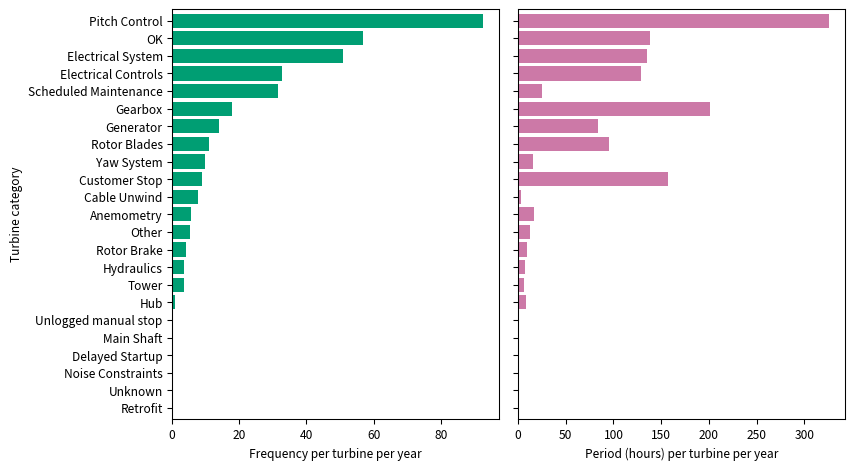
\includegraphics[width=\textwidth]{../images/f4}
  \caption{\label{f4}Bar chart showing the various turbine categories quantified by the downtime frequency per turbine per year on the left, and downtime period, in hours, per turbine per year on the right. This was plot using the downtime data.}
\end{figure}

\section{Performance of each class}

Since turbine category 10 was found to have the worst performance, the performance of each class for this label is looked at in more detail, which is done by obtaining confusion matrices. A confusion matrix displays, for each class, the number of samples predicted correctly and what the wrongly predicted samples were classified as \cite{33M}. This will allow the decision to be made whether the number of classes and intervals used for fault prediction can be tweaked for better classifier performance. The matrices were first obtained for all turbines with only this label using both imbalanced and balanced training data. Through five-fold cross-validation, a total of 125 matrices were produced, which were then combined and normalised, which will produce the classification accuracy. The confusion matrices are shown in \autoref{a4}. 93-95\,\% of `normal' and 73-75\,\% of `curtailment' samples were classed correctly. In comparison, only 21-24\,\% of `faulty' samples were classified correctly, with 47-48\,\% misclassified as `curtailment' and 21-26\,\% misclassified as `normal'.

Due to this misclassification percentage being higher than the accuracy of the `faulty' class, the classification was repeated by dropping all rows with `curtailment', effectively removing the class. There is a significant improvement in the accuracy of `faulty' samples, from 21-24\,\% to 41-44\,\%. However, the majority of samples belonging to this class (44-49\,\%) were still misclassified as `normal'. In fact, this is the case for the `X hours before fault' classes, with or without the use of the `curtailment' class. As X increases, the accuracy is seen to decrease, and the percentage of misclassification as `normal' increases.

To make a comparison, the same analysis was repeated for turbine category 5, which is `gearbox'. This category was chosen as its mean F1 score was relatively high (92\,\% compared to 84\,\% for turbine category 10), it causes the second longest downtime period based on \autoref{f4}, and it indicates a problem in the mechanical system, rather than electrical. 96-97\,\% of `normal' and 83\,\% of `curtailment' samples were classed correctly. In comparison, 43-44\,\% of `faulty' samples were classified correctly, with 16-21\,\% misclassified as `curtailment' and 34-40\,\% misclassified as `normal'. The performance was better compared to turbine category 10, but the misclassification of the `faulty' class as `normal' is higher. Removing the `curtailment' increased the accuracy of `faulty' samples, from 43-44\,\% to 48-55\,\%. However, the misclassification of this class as `normal' was still high (41-48\,\%).

Using a balanced dataset overall decreased the misclassification rate of `X hours before fault' classes as `normal', but increased the misclassification of the `faulty' class as `normal'.

\section{Feature importance}

The importance of each feature used, which are a set of normalised scores \cite{Rudy13}, were also obtained similar to the confusion matrix. The higher the feature importance, the more influence the feature had in determining the class of the samples. The feature importance for turbine categories 10 and 5 are shown in \autoref{t6}. For both turbine categories, the wind speed and nacelle position were found to be the most important features, and the maximum, average and deviations of the active power were found to be the least important, regardless of training data balancing. The wind direction was the third most important feature for turbine category 10 regardless of balancing, and for turbine category 5 using imbalanced data. In the case of balanced data for turbine category 5, the third most important feature was the pitch angle.

\begin{table}
  \centering
  \caption{\label{t6}Feature importance for turbine categories 10 and 5 using random forests and either imbalanced (I) or balanced (B) training data. The values are normalised and colour-coded, transitioning from red (lower importance) to yellow (intermediate) to green (higher importance).}
  \includegraphics[width=\textwidth]{../images/t6}
\end{table}

\chapter{Discussion}\label{c4}

As mentioned earlier, kNN compares the test sample to k neighbouring training
samples to determine the class. This means all training samples have to be
stored in memory \cite{Gutie} which in turn could slow down the computer,
causing the classifier to take a longer time to produce results. Being a
non-parametric technique \cite{16N} unlike DT and RF, kNN is prone to the
curse of dimensionality \cite{Gutie}, which happens when the dimensions or
number of features increases \cite{Distr}. This might explain the lower
performance metric scores in comparison. There are big differences between the
optimal k values for some turbines as shown in \autoref{f3} which could be due
to the data for each turbine having different distributions and
characteristics.

Overall, using a single multiclass-multilabel classifier with imbalanced
training data produced better scores, which could be due to presence of
correlations between the different turbine categories used as labels that are
generalised better using this approach \cite{110}.

As the labels `gearbox' and `electrical system' are in the top three out of 14
labels used causing longest downtimes, they should have more samples classed
as `faulty' and `X hours before fault' compared to other categories, which
therefore should result in better performance as the classifier would have
learned the characteristics of different samples belonging to the same
classes. This was not the case, however, looking at the confusion matrices in
\autoref{a4}. The classifier tends to misclassify `faulty' and `X hours before
fault' classes as `normal' at a higher rate than the accuracy for these
classes. This is still the case after removing the `curtailment' class, which
saw an improvement in the accuracy of the `faulty' class. The accuracies of
`X hours before fault' classes could potentially be increased by reducing the
6-hour intervals used and the maximum of 48 hours before a fault. The analysis
should be repeated by reducing 48 hours to a smaller timescale, such as 12
hours, or by combining all samples that fall under this with `faulty' points
to make the classification binary. Although this is likely to improve the
performance, the classifier will not be able to give an indication of the
timescale before a potential fault, therefore making it more difficult to
decide on the appropriate action to be taken to avoid catastrophic failure in
the turbine.

Based on the feature importance in \autoref{t6}, active power SCADA fields
were least influential in predicting faults for both labels. The labelled
power curves for `electrical system' in \autoref{f5} below shows no clear
relationship between fault points and the power curve shape. There are also
many overlapping `normal', `faulty' and `X hours before fault' points even
after filtration of curtailment and anomalies, which could explain why this
feature was less important.

\begin{figure}
  \centering
  \begin{subfigure}[t]{.5\textwidth}
    \centering
    \includegraphics[height=5cm]{../images/f5a}
    \caption{\label{f5a}}
  \end{subfigure}%
  \begin{subfigure}[t]{.5\textwidth}
    \centering
    \includegraphics[height=5cm]{../images/f5b}
    \caption{\label{f5b}}
  \end{subfigure}
  \begin{subfigure}[t]{.5\textwidth}
    \centering
    \includegraphics[height=5cm]{../images/f5c}
    \caption{\label{f5c}}
  \end{subfigure}
  \caption{\label{f5}Labelled power curve for turbine 1 with turbine category
  10 (`electrical system') through the two stages of filtering out anomalous
  and curtailment points labelled as `normal'. The original power curve is
  shown in \ref{f5a}. The first stage involves a filter based on a pitch angle
  threshold, which produces \ref{f5b}. The second stage involves several
  additional filters to produce the final power curve \ref{f5c}.}
\end{figure}

The reactive power and generator speed played a bigger role in the
classification for `electrical system', which makes sense considering the
reactive power is produced as a result of impedance in the current due to
electromagnetic fields produced by generators and transformers \cite{React}.
It is likely that the features used in classification for this label are
unsuitable. A fault in the electrical system would be reflected in voltages,
currents, frequencies \cite{Overb} and temperature of power switchboards and
cables. Electrical system faults could also be caused by environmental
conditions such as lightning strikes and contact of wires with wildlife
\cite{Overb}. If there are such conditions recorded as environmental downtime
categories, these should be accounted for when analysing faults in the
electrical system.

The `gearbox' label was also found to perform poorly for these classes,
despite having a higher mean F1 score than `electrical faults', which could be
due to feature selection as well. Statistics from the National Renewable
Energy Laboratory's gearbox failure database indicate that most faults are
caused by bearings, gears and other components including filtration and
lubrication systems \cite{Stati15}. These are mostly due to wear, fatigue and
cracks \cite{Sheng11} and may be detected with higher accuracy if the features
include quantities such as torque, oil pressure and gearbox temperature.

The SCADA data provided for this project only had 17 SCADA fields, of which 10
are used as features. This did not include voltages, currents, frequencies,
torques or temperature readings, but the SCADA system for the turbine model
used does measure these parameters. When a more complete SCADA data is
available, the evaluation should be done by increasing the number of features
to include these fields. The role of environmental conditions on failures
could explain why wind speed and direction were very influential in detecting
faults in the two labels analysed, although further in-depth analysis is
required to verify this.

Balancing the training dataset improved the classification accuracy of `X
hours before fault' classes slightly. An overall improved model may be
developed by oversampling only these classes for training, but there is a
trade-off between this and the training time and computational resources
required.

The dataset could have incorrect readings in the SCADA fields caused by broken
or unresponsive sensors which are not detected as unusual when the downtime
data is used in labelling. This was why a power threshold before cut-in speed
was applied to remove redundant data points, by visually inspecting the power
curve of the turbine as seen in \autoref{f1}. The dataset should be manually
inspected for all other features using curves such as pitch versus power and
power versus rotor speed, to see if there are any other incorrect values
previously undetected which may affect the classifier's accuracy in detecting
faults. The rows of data corresponding to these values should then be excluded
from the training data.

\section{Future Work}

In addition to possible areas for future work discussed above, the following
were identified.

When more data is available, the analysis should be repeated using historic
datasets spanning the life of the turbine. Historic data would have recorded
the different states a turbine has experienced over its life, and therefore
when a classifier is trained on this, it could detect future turbine states
easier. However, this will mean the training data will be bigger, which in
turn causes longer training time and more computing resources to be used.
Another area of work is to test the performance of a classifier using
different lengths of datasets for training while keeping the testing set and
hyperparameter settings constant. This will allow for the most appropriate
length of dataset for training to be determined based on the resources
available to produce satisfactory results in terms of training time and
classification accuracy.

After a classifier has been trained and used in practice, its performance over
time should be monitored. If the performance is found to diminish over time or
after a major component replacement, the classifier should be retrained using
recent data. As the classification makes a distinction between the different
faults, the ability to alert relevant maintenance professionals for a specific
fault automatically is possible.

Instead of using turbine categories in the downtime data, which is supervised,
for labelling, the alarm logs, which are unsupervised, can instead be used to
compare the results. The number of alarm logs for the turbines used, however,
is 480, compared to 23 turbine categories. This will mean the number of labels
will be much higher, which will cause longer computational time. A solution to
reduce this is to group similar alarms into one class. Another approach would
be to use a single label with each alarm as a separate class, but there is
likely to be overlap between classes when fault prediction is also included.
If actual failure records are available, a comparison can be made between the
predicted classes, actual classes, and actual failures that have occurred and
their costs.

Further optimisation of hyperparameters is possible, such as finding the
optimal number of estimators for RF. Each optimisation takes time and is
limited by the specifications of the computer used, which is why this was not
carried out in this project. Detailed analysis done on the results using RF
for two labels above should be repeated for each label and classifier used for
fair comparisons to be made.

The methodology could also be tested for wind turbines of different models in
different sites. Provided these turbines have similar SCADA data with downtime
records, only slight modifications to the codes, such as the data source,
field names, and number of features, would be required in order to be used on
other turbine models.

In industry, a cost function analysis needs to be done prior to implementing
this fault detection method. It is defined as the cost of a false alarm (false
positive) or failing to detect a fault in advance (false negative). False
positives and false negatives both incur charges. The first is due to
transporting labour and equipment to site, which could be expensive especially
for sites in harsh environments, such as offshore wind farms. The second would
cause unscheduled downtime, the loss of revenue due to no power generation and
replacement of turbine components due to irreversible damage. This cost should
then be compared to the cost of alternatively using a condition monitoring
system, and the overall cost of running the wind farm or wind turbine. The
analysis should give an indication on which performance metric is more
important; if the cost of false negatives is more, attention should be paid to
the recall score, while the precision is more important if false positives
cost more \cite{deRu15}.

\chapter{Conclusion}\label{c5}

A methodology for predicting multiple wind turbine faults in advance by implementing classification algorithms on wind turbine SCADA signals was proposed. 30 months' worth of SCADA data for a wind farm with 25 turbines was processed and labelled using corresponding downtime data containing turbine categories that describe the condition of the turbine. Since the multiple faults are treated as separate labels, multiclass-multilabel classification algorithms, namely DT, RF and kNN, offered in scikit-learn, the machine learning library for Python, were analysed. In order to predict faults in advance, three types of classes were used: `normal' to indicate normal behaviour, `faulty' to indicate a fault, and `X hours before fault' (where X $=$ 6, 12, \dots, 48) to detect faults in advance at varying time scales. This will allow predictive maintenance to be done appropriate to the time scale to prevent catastrophic failure to the turbine. Each of these classifiers have hyperparameters which were tuned for optimal performance on the data using five-fold cross-validation. The effects of balancing training data were also investigated.

The use of multilabel-multiclass algorithms allowed for the classification of each turbine to be done using a single estimator which produces the results of all labels simultaneously and has a shorter training time. Of the three classifiers, RF was found to have the best performance overall. A detailed analysis was done on the results for two labels, namely `electrical system', which had the worst performance, and `gearbox' which had relatively better performance. The performance of the `X hours before fault' classes was found to be relatively poor compared to the other two classes. The performance of these classes was slightly better using balanced training data. This has drawbacks, including using separate estimators for each label, and increased training time and use of resources due to the use of larger training data. After evaluating feature importance, it was concluded that the poor performance of these classes could be attributed to the features used or errors in the data. Further work should be done using additional SCADA fields relevant to each label to verify this. After additional improvements to the model and conducting a cost function analysis, the method could be tested in industry.


{%
  \backmatter%
  \chapter{Acknowledgements}

I would like to thank my academic supervisor, Dr Nick Bennett, Assistant Professor at HeriotWatt University, and my industrial supervisor, Dr Iain Dinwoodie, Senior Asset Performance Engineer at Natural Power, for their endless guidance and feedback, and making this project possible. Special thanks to the Technical team of Natural Power for giving me the opportunity to work on this project with them. Thanks to everyone else at Natural Power's Stirling office and my course mates, Raphaela Hein and Inés Ontillera, for making this placement an enjoyable experience. Last but not least, a big thank you to my parents for supporting me throughout my studies.
%
  \chapter{References}%
  \printbibliography[heading=none]%
}

\theappendix
\chapter{Pitch angle threshold}\label{a1}

\begin{figure}
  \centering
  \begin{subfigure}[t]{.5\textwidth}
    \centering
    \includegraphics[height=4.8cm]{../images/fa1a}
    \caption{}
  \end{subfigure}
  \begin{subfigure}[t]{.5\textwidth}
    \centering
    \includegraphics[height=4.8cm]{../images/fa1b}
    \caption{}
  \end{subfigure}
  \begin{subfigure}[t]{.49\textwidth}
    \centering
    \includegraphics[height=4.8cm]{../images/fa1c}
    \caption{}
  \end{subfigure}
  \begin{subfigure}[t]{.49\textwidth}
    \centering
    \includegraphics[height=4.8cm]{../images/fa1d}
    \caption{}
  \end{subfigure}
  \captionsetup{labelformat=empty,list=no}
  \caption{Power curves for turbine 1 used in selecting the pitch angle threshold. a is the original power curve. In b, data points with a pitch angle not equal to 0\,\textdegree between 90\,\% and 10\,\% power were filtered out, which distorts the power curve shape. In c, all data points have a pitch angle between 0\,\textdegree and 3.5\,\textdegree, which removes most curtailment and anomalous points while maintaining the typical power curve shape. In d, all data points have a pitch angle between 0\,\textdegree and 7\,\textdegree, which allows some curtailment points to appear. Therefore, it was decided that the filter used in c is the most suitable.}
\end{figure}

\chapter{Power before cut-in threshold}\label{a2}

\begin{figure}
  \centering
  \begin{subfigure}[t]{.5\textwidth}
    \centering
    \includegraphics[height=5cm]{../images/fa2a}
    \caption{}
  \end{subfigure}
  \begin{subfigure}[t]{.5\textwidth}
    \centering
    \includegraphics[height=5cm]{../images/fa2b}
    \caption{}
  \end{subfigure}
  \captionsetup{labelformat=empty,list=no}
  \caption{Power curves for turbine 24 used in selecting the power threshold before cut-in speed. a is the original power curve. b is the power curve with a filter applied to remove all data points with power > 0 kW before the cut-in speed of 3 m/s. Anemometer wind speeds, which were used to plot these power curves, are not an accurate measure of the wind speed incident on the turbine blades. Therefore, a threshold of 100 kW before cut-in is applied, which maintains the power curve shape for all 25 turbines while removing anomalous points, such as the ones in turbine 2's power curve.}
\end{figure}

\chapter{Results for random forest classifier}\label{a3}

\begin{landscape}
  \begin{table}
    \centering
    \captionsetup{labelformat=empty,list=no}
    \caption{Precision, recall and F1 scores for each turbine using random forest classifier for both imbalanced and balanced training data. The table lists the minimum, mean and maximum values for each score, which are also colour-coded to show higher scores in darker shades and lower scores in lighter shades.}
    \includegraphics{../images/ta1}
  \end{table}
\end{landscape}

\begin{table}
  \centering
  \captionsetup{labelformat=empty,list=no}
  \caption{Precision, recall and F1 scores for each turbine category using random forest classifier for both imbalanced and balanced training data. The table lists the minimum, mean and maximum values for each score, which are also colour-coded to show higher scores in darker shades and lower scores in lighter shades.}
  \includegraphics{../images/ta2}
\end{table}

\chapter{Confusion matrices}\label{a4}

\begin{table}
  \centering
  \captionsetup{labelformat=empty,list=no}
  \caption{Normalised confusion matrices for turbine category 10 (`electrical system') with all classes used in the classification process using random forests and either imbalanced or balanced training data. The matrix is colour-coded; it transitions from red (lower scores) to yellow (intermediate) to green (higher scores).}
  \includegraphics[width=.99\textwidth]{../images/ta3}
\end{table}

\begin{table}
  \centering
  \captionsetup{labelformat=empty,list=no}
  \caption{Normalised confusion matrices for turbine category 10 (`electrical system') when classification is done using random forests and either imbalanced or balanced training data without the `curtailment' class (i.e., rows of data with curtailment or anomalies in any label are dropped). The matrix is colour-coded, transitioning from red (lower scores) to yellow (intermediate) to green (higher scores).}
  \includegraphics{../images/ta4}
\end{table}

\begin{table}
  \centering
  \captionsetup{labelformat=empty,list=no}
  \caption{Normalised confusion matrices for turbine category 5 (`gearbox') with all classes used in the classification process using random forests and either imbalanced or balanced training data. The matrix is colour-coded; it transitions from red (lower scores) to yellow (intermediate) to green (higher scores).}
  \includegraphics[width=.99\textwidth]{../images/ta5}
\end{table}

\begin{table}
  \centering
  \captionsetup{labelformat=empty,list=no}
  \caption{Normalised confusion matrices for turbine category 5 (`gearbox') when classification is done using random forests and either imbalanced or balanced training data without the `curtailment' class (i.e., rows of data with curtailment or anomalies in any label are dropped). The matrix is colour-coded, transitioning from red (lower scores) to yellow (intermediate) to green (higher scores).}
  \includegraphics{../images/ta6}
\end{table}

\chapter{Python code}\label{a5}

Python code used in this project can be found in its GitHub repository, which can be accessed through the following link: \url{https://github.com/nmstreethran/WindTurbineClassification}.


%%%%%%%%%%%%%%%%%%%%%%%%%%%%%%%%%%%%%%%%%%%%%%%%%%%%%%%%%%
\end{document}
